\chapter{Results and Analysis}

\section{Simulated Data}

\subsection{Test Cases}

The test cases looked at were selected to determine the effects of the spacecraft inertia, the spacecrafts orbit and its geometry. In Total 18 total cases were simulated, each simulated at various times of the year with randomized angular velocities.

The geometries used in this analysis were a rectangular prism, a cylinder, and a box-wing. The first two are convex geometries that have differing levels of symmetry, while the box-wing geometry is concave. The orbits examined are Low Earth Orbits (LEO), Medium Earth Orbits (MEO) and Geostationary Earth Orbits. The final variable is the spacecrafts inertia. In the first case, the pricipal inertial axes are assumed to be aligned with the spacecraft body frame and equal. The effect of this is to make the spin axis constant for all time. In the second case, the principal inertial axes are all different and are not aligned with the body frame, causing the spin axis to change over time.

\begin{figure}\label{simulated_geometries}
	\begin{center}
	\begin{tabular}{cc}
		\includegraphics[width = 50mm]{Long_Rectangle_Image_Axes.png} &
		\includegraphics[width=50mm]{Cylinder_Axes} \\
		Rectangular Prism & Cylinder \\
		\multicolumn{2}{c}{\includegraphics[width=50mm]{Box_Wing_Axes}} \\
		\multicolumn{2}{c}{Box Wing}
	\end{tabular}
	\end{center}
	\caption{Three Simulated Geometries.}
\end{figure}


\begin{figure}
	\begin{center}
	\begin{tabular}{cc}
		\includegraphics[width = 50mm]{leo_orbit} &
		\includegraphics[width=50mm]{meo_orbit} \\
		Low Earth Orbit (465km x 506km) & Medium Earth Orbit (541km x 21,200km) \\
		\multicolumn{2}{c}{\includegraphics[width=50mm]{geo_orbit}} \\
		\multicolumn{2}{c}{Geostationary Orbit (35,786km x 35,786km)}
	\end{tabular}
	\end{center}
	\caption{Three Simulated Orbits.}
\end{figure}

\subsection{Methodology}

\subsubsection{Simulation Methodology}
First, a LEO, MEO, and GEO orbit were selected. Passes were calculated by brute force sampling a spacecrafts location and checking for necessary conditions. These conditions were obviously that the spacecraft must be above the horizon of the observation site and that the spacecraft be illuminated. Passes lower than 20 degrees elevation were discarded. Additionally, in preliminary experiments it was noticed that the UKF often failed to converge to a solution when the angle between the observation and sun vector was greater than 90 degrees. Therefore passes whose observation and sun vectors were speparated by more than 90 degrees were also discarded. Passes were also limited to only 5 minutes of data collection as MEO spacecraft passes can be hours long and geostationary passes are perpetual.

Once a pass was identified, the spacecraft was given three initial attitudes and angular velocities between 0.1 and 0.3 radians per second. These were then propagated and used to calculate three different light curves per pass. Before entering the Kalman Filter, Gaussian noise was added to the light curve whose distribution was similar to that of the real data collected. The standard deviation seen in the real data varied typically between 1-30 counts, and so this range of values was used to generate the gaussian noise.

The simulated sample rate was 100 measurements per second or 0.01 seconds between measurements. This is significantly higher than the sample rates used by other researchers such as one sample every 1.316 seconds in Wetterer et. al \cite{wetterer_ukf} or one every 5 seconds in Holzinger et. al \cite{Holzinger2012AttitudeEF}. This was done to match the data provided by Lockheed-Martin which contained a range of sample rates which were typically in the neighborhood of one sample every 0.02 seconds. This is quite remarkable.

The inertia matrix used for the spacecraft in the tumbling cases was as follows:
\begin{equation}
\begin{bmatrix}
1 & .01 & .01 \\ .01 & 2 & .01 \\ .01 & .01 &3
\end{bmatrix}
\end{equation}
With the exception of the MEO and GEO box wing tumbling cases whose off-diagonal elements were set to zero.

This matrix follows the assumption used in the derivation of the UKF formulation which was that the off-diagonal elements are small and therefore negligible. It should be noted that the formulation used to estimate these parameters does not estimate the offdiagonal elements.

Both UKFs were initalized with an angular velocity of $[0.01, 0.01, 0.01]$ and an initial Modified Rodriguez Parameter of $[0.01, 0.01, 0.01]$. The diagonal inertia terms were initially set to $[1, 1]$.

No differences were added to the geometric models between the data simulation and UKF analysis.

\subsubsection{Convergence Criteria}

Convergence was determined by examining the magnitude of the update to the angular velocity. If it was seen that the angular velocity was updated on average less than 1e-4 radians/second then it was said to have converged. For the real data the threshold of 2e-3 was applied to determine convergence.

For the cases where angular velocity was held constant, this resulted in very satisfactory results. However, in the cases where the angular velocity was not constant, the UKF would meet the convergence criteria without producing a realistic solution. The successful runs of the UKF for these cases were then hand selected using the criteria that a valid solution for angular velocity should appear sinusoidal and not change dramatically in amplitude or period.

This is likely due to the UKF's forumation as it is unable to completely estimate the inertia matrix. Therefore even when it converges to the correct angular velocity it deviates from this over time requiring relatively large update steps.

\subsubsection{Data Filtering}

When analyzing the data it is important to keep in mind that this problem is indeterminate and that multiple solutions are possible which are all equally plausible when the objects true attitude is not known. This poses a challenge in quantifying the performance of the UKF as the result can only be directly compared to the simulated truth when the UKF happens to converge to it rather than another equally plausible solution. When the UKF produces one of these alternate solutions, it cannot be compared to the simulated truth to measure accuracy. This would not be an issue if these alternate solutions were the minority of solutions found as they could simply be discarded. However, these alternative solutions are by far the majority.

A known example of a solution which can never be discarded is the angular velocity corresponding to the negative of the truth. It is not possible to know whether an object spins clockwise or counterclockwise about any given axis using only light curve data \cite{Spin_Direction}. Therefore, in this thesis, only the axis of rotation is examined. What this means is that, during analysis, the estimated angular velocity was multiplied by 1 or -1 to minimize the dot product between the true angular velocity and estimated angular velocity. This simply serves to make valid results more apparent.

\begin{figure}[ht]\label{awful_errors}
	\begin{center}
		\includegraphics[width = 85mm]{figures/ECI_percent_errors}
		\caption{Relative Error in the ECI Frame When Directly Comparing to Simulated Truth}
	\end{center}
\end{figure}

As can be seen in figure \ref{awful_errors} by simply comparing the converged solution with the truth model the performance appears to be lousy. This does not make sense, as every converged solution successfully recreated the simulated lightcurve, meaning that it is a completely plausible solution.

What was assumed is that for any given simulted trial, for every axis there are multiple valid solutions and that if the data were filtered many times these solutions would each appear as a group of solutions centered on a mean with similar variances. A hypothetical example of this is shown in figure \ref{distributions}. This assumptions may not be valid. It may me that the solutions overlap significantly and it is not possible to separate them. However, in genal once the UKF settled on a solution it showed a very small variance, making it likely that this assumption is true.

\begin{figure}[ht]\label{distributions}
	\begin{center}
		\includegraphics[width = 85mm]{figures/Assumptions_Example}
		\caption{Hypothetical Results for Multiple Trials}
	\end{center}
\end{figure}

In order to yield meaningful results without reducing the sample size to only a handful of cases, the following methodology was applied to the data. \textbf{If any component of the angular velocity fell within 3 standard deviations of the ground truth, it was considered to be converging towards it and its error would be added to the statistics. This allows for an analysis to be conducted but does reduce the strength of the results.}

\subsubsection{The Observation Frame}

Angular velocities were analyzed in two frames: The body frame and the observation frame. The body frame is the reference frame fixed to the spacecraft body. In this frame, direct comparisons can be made to the ground truth and deductions can be made about performance with respect to the spacecraft geometry. As it can be shown that multiple attitudes can result in the same light curve, the body frame serves as a poor frame to analyze angular velocities which may appear wildly different in body frame but which closely mirror the ground truth when the spacecraft attitude is accounted for. The best frame to analyze this is the Observation frame.

\begin{figure}[ht] \label{body errors}
	\begin{center}
		\includegraphics[width = 65mm]{figures/Observation_Frame.png}
		\caption{Definition of the Observation Frame With Respect to the Sun and Observation Vectors.}
	\end{center}
\end{figure}

The observation frame is defined to have its origin at the center of the spacecraft, its X axis along the observation vector, the Z axis being the cross of the sun and observation vector, and the Y axis completing the frame. This frame enabled comparisons between the estimated and true angular velocities in a frame which is irrespective of the spacecrafts attitude. Additionally, this frame allows for the error analysis with respect to the geometry of the situation. E.g, the direction of observation and illumination with respect to the spacecraft.

\subsection{Simulation Results}

\subsubsection{Existence of Multiple Solutions}
The simulation results reveal that the problem of uniquely identifying an attitude profile from a light curve is an indeterminate problem. The data shows that for any light curve, there are multiple combinations of attitude profiles and angular velocities that can produce it. Many of these solutions are a result of the symmetry of the spacecraft. 

The number of indistinguishable solutions could be reduced if the observed object has a highly asymmetric geometry or if its reflectance properties vary between panels. These two quantities both depend on the object and can be conveniently selected in simulations, however in reality many objects are highly symmetrical and the reflectance properties across the geometry would be unknown.

After seeing these results, one final run was conducted using the rectangular prism geometry in a geostationary orbit with each face having different reflactance properties. What was found was that the convergence success rate increased to 83\%, however only 1 solution in 36 converged exactly to the simulated truth.

It should be carefully considered when selecting the reflectance properties of the spacecraft without complete knowledge. Any light curve can be recreated using any combination of geometry and reflectance properties \cite{Spin_Direction}. Attempting to reduce the number of solutions in this way without knowledge of the true properties may result in the exclusion of correct solutions.

\subsubsection{Hypothesis}

This thesis hypothesizes that a predicable set of solutions exists which can recreate a given lightcurve. This second set of solutions is characterized by an angular velocity vector whose magnitude and direction are directly mirrored across the XY plane of the observation frame.

It can be noticed in the formulation of the measurement model that measured light intensity is a function of the relative directions of the facet normals, observation, and velocity vectors. If sufficient symmetry exists within the spacecraft geometry such that it is possible to create what appears to be a reflection of the spacecraft geometry though only rotation, then this second set of solutions is expected to exist. This is because a mirroring of the spacecraft geometry about the XY plane of the observation frame preserves the angles between the sun, observation, and each facet normal vector.

This is only possible when the observational plane remains relatively constant however. As the observational plane changes, so must the mirrored angular velocity. As the UKF used in this thesis assumes that the angular velocity is either constant or changes according to Eulers equations of rigid body motion. This un-modeled motion usually excludes the mirrored solution as valid.


\subsubsection{Case: Fixed Axis of Rotation}

\begin{table}[ht]
	\begin{center}
		\begin{tabular}{| c | c | c | c | c |}
			\hline Geometry & LEO & MEO & GEO & Total Trials\\ 
			\hline Cylinder & 52.77\% & 48.88\% & 69.44\% & 117 \\
			\hline Rectangular Prism & 19.44\% & 57.77\% & 63.88\% & 117\\
			\hline Box-Wing & 0.00\% & 50.00\% & 86.95\% & 80\\
			\hline
		\end{tabular}
	\end{center}
	\caption{Percentages of Trials with Converged Solutions: Fixed Axis Case}
\end{table}

\begin{figure}[ht]
	\begin{center}
		\includegraphics[width = 85mm]{Body_Errorbars}
		\caption{Angular Velocity Error by Body Axis and Geometry With Data Filtering}
	\end{center}
\end{figure}

\begin{figure}
	\begin{tabular}{cc}
		\includegraphics[width = 65mm]{figures/Rectangle_Leo/BODY} &
		\includegraphics[width=65mm]{figures/Rectangle_Leo/CURVE} \\
		Angular Velocity in Body Frame & Light Curve Comparison \\
		\includegraphics[width = 65mm]{figures/Rectangle_Leo/OBS} &
		\includegraphics[width = 65mm]{figures/Rectangle_Leo/MRP} \\
		Angular Velocity in Observation Frame & Modified Rodrigues Parameter Comparison
	\end{tabular}
	\caption{Converged Solution of a Rectangular Prism in LEO spinning About a Fixed Axis.}
\end{figure}


\begin{figure}
	\begin{tabular}{cc}
		\includegraphics[width = 65mm]{figures/Cylinder_Leo/BODY} &
		\includegraphics[width=65mm]{figures/Cylinder_Leo/CURVE} \\
		Angular Velocity in Body Frame & Light Curve Comparison \\
		\includegraphics[width = 65mm]{figures/Cylinder_Leo/OBS} &
		\includegraphics[width = 65mm]{figures/Cylinder_Leo/MRP} \\
		Angular Velocity in Observation Frame & Modified Rodrigues Parameter Comparison
	\end{tabular}
	\caption{Converged Solution of a Cylinder in LEO Spinning About a Fixed Axis.}
\end{figure}

\begin{figure}
	\begin{tabular}{cc}
		\includegraphics[width = 65mm]{figures/BW_Geo/BODY} &
		\includegraphics[width=65mm]{figures/BW_Geo/CURVE} \\
		Angular Velocity in Body Frame & Light Curve Comparison \\
		\includegraphics[width = 65mm]{figures/BW_Geo/OBS} &
		\includegraphics[width = 65mm]{figures/BW_Geo/MRP} \\
		Angular Velocity in Observation Frame & Modified Rodrigues Parameter Comparison
	\end{tabular}
	\caption{Converged Solution of a Box-Wing in GEO Spinning About a Fixed Axis}
\end{figure}

The first result is that the UKF performs significantly better in the Geostationary cases. Excepting the cylinder case, where the LEO and MEO had similar success rates, it seems that LEO is the most challenging for the UKF.

This is likely due to the fact that in both MEO and LEO, the amplitude of the light curve can vary dramatically across the pass as the objects distance from the observer changes. This means that small errors in the state estimate correspond to different magnitude errors depending on when they occur during the pass. This is to say that the model uncertainty changes throughout the pass while the UKF assumes it is constant. The reason MEO performs better than LEO is because a MEO object near apogee has a very constant amplitude. In GEO, the spacecraft effectively do not change their distance from the observer and so their model uncertainty remains extremely constant.

It can be see that in the body frame, the cylinder geometry had significantly better performance about its Z-axis which corresponds to its length. In figure \ref{simulated_geometries} it can be seen that the cylinder is modeled as a set of flat facets. It is likely that as the number of facets increases that the error along the Z axis also increases. This is because as the cylinder rotates each facet brightens and then dims, creating bumps in the intensity signal that would not be caused by a true cylinder. These bumps very likely make it easier for the UKF to converge on the Z axis angular velocity. As the number of facets increases, the effect of these bumps is expected to vanish.

In general the box-wing geometry has large error compared two the other two. It is likely that the significantly reduced error about the Y axis has to do with the placement of the panels. The Y axis of this geometry corresponds to the axis normal to the "wings". The box-wing geometry was also the smallest geometry and so the modeled noise affected the signal proportionately more, which would explain the overall higher uncertainty for this geometry.

\begin{figure}[ht] \label{obs errors}
	\begin{center}
		\includegraphics[width = 85mm]{OBS_Errorbars}
		\caption{Angular Velocity Error by Observation Frame Axis and Geometry With Data Filtering}
	\end{center}
\end{figure}

Looking that the error in the Observation Frame performance in figure \ref{obs errors}, the cylinder geometry performed significantly better than the other two. Potentially this is due to the fact to make large changes in the attitude without affecting the performance by changing its rotation about its Z body axis. This decoupling between atitude and lightcurve may decrease the potential for this geometry to become stuck in a local minimum.



\subsubsection{Case: Tumbling Spacecraft}

\begin{table}[H]
	\begin{center}
		\begin{tabular}{| c | c | c | c | c |}
			\hline Geometry & LEO & MEO & GEO & Total Trials\\ 
			\hline Cylinder & 22.00\% & 25.00\% & 25.00\% & 108 \\
			\hline Rectangular Prism & 2.77\% & 2.77\% & 16.66\% & 108\\
			\hline Box-Wing & 0.00\% & *0.00\% & *41.37\% & 101\\
			\hline \multicolumn{5}{c}{* Spacecraft truth model had no off-diagonal elements.} \\
			\hline
			
		\end{tabular}
	\end{center}
	\caption{Percentages of Trials with Converged Solutions: Tumbling Case}
\end{table}

\begin{figure}
	\begin{tabular}{cc}
		\includegraphics[width = 65mm]{figures/Cylinder_Meo_Tumbling/BODY} &
		\includegraphics[width=65mm]{figures/Cylinder_Meo_Tumbling/CURVE} \\
		Angular Velocity in Body Frame & Light Curve Comparison \\
		\multicolumn{2}{c}{\includegraphics[width=65mm]{figures/Cylinder_Meo_Tumbling/INERTIA}}\\
		\multicolumn{2}{c}{Estimated Inertia Values}
	\end{tabular}
	\caption{Converged Solution of a Cylinder in MEO Tumbling.}
\end{figure}

\begin{figure}
	\begin{tabular}{cc}
		\includegraphics[width = 65mm]{figures/Rect_Meo_Tumbling/BODY} &
		\includegraphics[width=65mm]{figures/Rect_Meo_Tumbling/CURVE} \\
		Angular Velocity in Body Frame & Light Curve Comparison \\
		\multicolumn{2}{c}{\includegraphics[width=65mm]{figures/Rect_Meo_Tumbling/INERTIA}}\\
		\multicolumn{2}{c}{Estimated Inertia Values}
	\end{tabular}
	\caption{Converged Solution of a Rectangular Prism in MEO Tumbling.}
\end{figure}


\begin{figure}
	\begin{tabular}{cc}
		\includegraphics[width = 65mm]{figures/BW_Geo_Tumbling/BODY} &
		\includegraphics[width=65mm]{figures/BW_Geo_Tumbling/CURVE} \\
		Angular Velocity in Body Frame & Light Curve Comparison \\
		\multicolumn{2}{c}{\includegraphics[width=65mm]{figures/BW_Geo_Tumbling/INERTIA}}\\
		\multicolumn{2}{c}{Estimated Inertia Values}
	\end{tabular}
	\caption{Converged Solution of a Box-Wing in GEO Tumbling.}
\end{figure}

The success rates for the tumbling cases were far lower than in the fixed axis case. This is to be expected however as the number of parameters to estimate and the complexity of the models are significantly greater. Again though, we see the pattern in which performance increases with orbital altitude.

Another trend which has continued into the tumbling case is that there are once again multiple solutions which result in the same predicted measurement. In this new data we see solutions converging with variations in period and amplitude in addition to magnitude and direction. These extra degrees of freedom could potentially be why the UKF struggles to settle on a single solution.

In regards to the Inertia estimation, results varied wildly. It is known that in the absence of disturbances only the relative magnitude of the inertia values matter. The top left element was forced to be 1, and the other two diagonal elements were expected to converge to the true values. What was seen in the data however was that the inertia values often converged to values which differed from the truth, but preserved the same ratios between inertial axes.




\subsubsection{Hypothesis Results}

By examining the angular velocities in the observation frame, it was observed that 6 of the 117 trials converged to a solution which was mirrored across the observational plane. This was apparent because, in the observation frame, the angular velocity converged to the correct axis and magnitude with the exception that the Z component was the negative of what the truth.

\begin{figure}[ht]\label{flipped_obs}
	\begin{tabular}{cc}
		\includegraphics[width = 65mm]{figures/flips/R_OBS} &
		\includegraphics[width=65mm]{figures/flips/R_CURVE} \\
		Angular Velocity in the Observation Frame & Light Curve Comparison
	\end{tabular}
	\caption{Example of a solution which is flipped across the observation plane.}
\end{figure}

\begin{figure}[ht]\label{flipped_frames}
	\begin{center}
		\includegraphics[width=140mm]{figures/flips/R_FRAMES}
	\end{center}
	\caption{Consecutive Images from the observers perspective of truth [TOP] and estimate [BOTTOM] showing a mirror image solution.}
\end{figure}

In figure \ref{flipped_obs} it can be see that the angular velocity estimate converges to ground truth except for along the Z axis, where it converges to the negative. This corresponds with a mirroring of the angular velocity about the XY plane of the observation frame.

In figure \ref{flipped_frames} a visualization is shown of the truth and estimated spacecraft attitudes. Here the symmetrical relationship between the true attitude and its mirrored counterpart.

Additionally, it can be seen in figure \ref{flipped_frames} that the light curve is nearly identical to the original, suggesting that these two solutions are indistinguishable.

This result is important because as there are so many ways in which this attitude estimation problem are indeterminate. Any way in which a result can be predictably associated with a set of other potential solutions significantly increases the utility of the analysis. Knowing that this additional solution is possible allows for any single solution to now represent at least 4 alternative solutions which are simple transformations of each other. These 4 solutions are then the true angular velocity, its reflections, and their negatives.

\section{Real Data}

\subsection{Real vs Simulated Data}

It is noted that the real data looks significantly different than the simulated data. The simulated data has clearly defined, macroscopic, periodic variations which can clearly be attributed to a rotating, reflecting surface. The real data, which can be seen in Appendix B., is much more ambiguous. It is unknown if the high frequency variations in the data are noise or signal. A Fourier transform of the data did not show any frequency begin significantly dominant.

The UKF largely ignored this high frequency variation and instead appeared to track the mean.

\subsection{SERT-2}

The Space Electric Rocket Test II (SERT-2) is a modified Aegena rocket body whose mission was to test two ion propulsion systems on board. \cite{sert2} In order to power these propulsion systems, two deployable solar panels were added to the Aegena rocket body whose dimensions were 1.5x6 meters. The dimensions of the Aegena module were also 1.53x6 meters.

SERT-2 was launched on February 3rd, 1970 and was finally decommissioned in 1991. Due to the age of the spacecraft and considering that there is potentially fuel remaining within the Aegena tank, this spacecraft can be assumed to be spinning about its major axis. This obviously simplifies the UKF model and allows this thesis to implement the simpler version.

The geometry of SERT-2 is essentially a cylinder with two rectangular panels radiating from one end. This model is non-convex which means that it can take advantage of ray tracing algorithm described in this thesis. 

\begin{figure}\label{sert_model}
	\begin{tabular}{cc}
	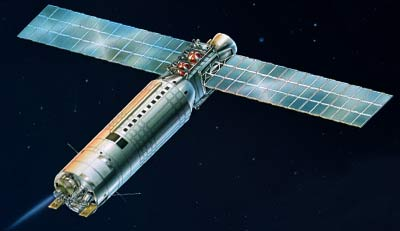
\includegraphics[width = 80mm]{figures/sert-2} & \includegraphics[width = 60mm]{figures/SERT2_Axes} \\
	SERT-2, Source: NASA & SERT-2 Reflectance Model 
	
	\end{tabular}
	\caption{SERT-2 vs Reflectance Model}
\end{figure}

\begin{figure}
	\begin{tabular}{cc}
		\includegraphics[width = 50mm]{figures/Sert_Success/BODY} &
		\includegraphics[width=50mm]{figures/Sert_Success/CURVE} \\
		Angular Velocity in Body Frame & Light Curve Comparison \\
		\includegraphics[width = 50mm]{figures/Sert_Success/ECI} &
		\includegraphics[width = 50mm]{figures/Sert_Success/MRP} \\
		Angular Velocity in ECI Frame & Modified Rodrigues Parameter Estimates
	\end{tabular}
	\caption{Convergence of a solution using real data of SERT-2.}
\end{figure}

The geometric model for SERT-2 can be see in figure \ref{sert_model}. The reflectance properties used for each panel were a specular reflectance of 0 and a diffuse reflectance of 0.002 . This reflectance is unrealistically low as the average albedo for fragmentation debris is closer to 0.152 \cite{global_albedo}. The practical effects of this discrepancy is that the magnitude of the measurement model output is scaled by about two orders of magnitude compared to if a resonable value had been used.

Obviously there is nothing to compare these estimates with as the true angular velocity of SERT-2 is unknown. However, in figure \ref{sert_table} the angular velocity and measurement dates are reported for the successful trials. It is possible that since SERT-2 has been in orbit for now five decades, its possible that its angular velocity has settled into stable configuration. As the data analyzed were collected only days apart it is possible that, similar results would be observed in the ECI frame. However, this thesis found no discernible pattern with respect to the ECI results.

It is interesting to note that in the body frame, the majority of the solutions show SERT-2 primarily spinning about its Z axis.

% Table generated by Excel2LaTeX from sheet 'datatable'
\begin{table}[htbp]\label{sert_table}
	\centering
	
	\begin{tabular}{|l|r|r|r|r|r|r|}
		\hline Measurement Date & X Body & Y Body & Z Body & X ECI & Y ECI & Z ECI \\
		\hline 2018-06-02 & -0.03838 & 0.099123 & 0.276464 & -0.03607 & -0.20629 & -0.20946 \\
		\hline 2018-06-15 & 0.094913 & 0.307434 & -0.29946 & 0.4386 & -0.0136 & 0.025415 \\
		\hline 2018-06-23 & -0.0934 & -0.0615 & 0.547375 & 0.448295 & -0.31579 & -0.10693 \\
		\hline 2018-06-27 & 0.004656 & -0.00586 & -0.58329 & 0.29951 & -0.38325 & 0.322009 \\
		\hline 2018-07-02 & 0.012748 & 0.02757 & -0.68151 & -0.08979 & -0.67597 & -0.01929 \\
		\hline 2018-07-07 & 0.107008 & 0.096465 & 0.264944 & 0.206755 & -0.21221 & -0.05632 \\
		\hline 2018-07-16 & -0.00967 & -0.75654 & -0.00129 & -0.53145 & 0.385914 & -0.37562 \\
		\hline 2018-08-10 & -0.06039 & 0.011915 & 0.613305 & -0.33712 & 0.489952 & 0.161957 \\
		\hline 
	\end{tabular}%
	\caption{Final Angular Velocity Vector of SERT-2 According to UKF Estimates.}
\end{table}%



\subsection{Ajisai (EGS)}

Ajisai was a mission launched on August 13th, 1986 and was primarily intended as a dummy payload for the H-I launch vehicle. \cite{ajisai_jaxa} Ajisai is essentially a sphere covered with 1,436 corner cube reflectors and 318 mirrors. \cite{ajisai} Its secondary mission (after being mass) was to determine the exact position of the more isolated Japanese islands. \cite{ajisai_jaxa}

Because this spacecraft is so old and because it is a sphere. It is highly likely that it is spinning about its major axis and the simpler UKF formulation can be applied once more.

\begin{figure}[!ht]
	\begin{tabular}{cc}
	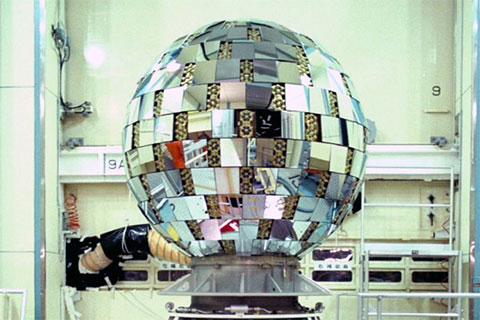
\includegraphics[width = 90mm]{figures/ajisai.jpg} & \includegraphics[width = 60mm]{figures/AJISAI_Axes} \\
	AJISAI, Source: JAXA & AJISAI Reflectance Model
	\end{tabular}
	\caption{AJISAI vs Reflectance Model}
\end{figure}



The geometry of the spacecraft is simply a large set of reflective panels. Being mirrors, these panels will have very high specular reflectance and almost no diffuse reflectance. The corner cube reflectors designed to reflect light back to its source. For this thesis, that source is the sun, and so the corner cube reflectors can be assumed to contribute nothing to the lightcurve. Thankfully, the positions of each corner cube reflector were documented, and the panel locations can be inferred from them.

\begin{figure}
	\centering
	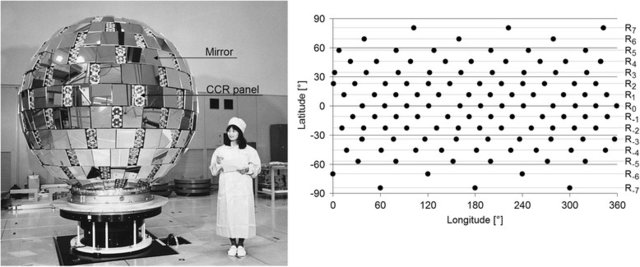
\includegraphics[width = 150mm]{figures/ajisai_panels.jpg}
	\caption{AJISAI with Engineer [Left]. Corner Cube Reflector Locations [Right] \cite{ajisai}}
\end{figure}

\begin{figure}[!ht]\label{ajisa_fail}
	\begin{tabular}{cc}
		\includegraphics[width = 50mm]{figures/Ajisai_Fail/BODY} &
		\includegraphics[width=50mm]{figures/Ajisai_Fail/CURVE} \\
		Angular Velocity in Body Frame & Light Curve Comparison \\
		\includegraphics[width = 50mm]{figures/Ajisai_Fail/ECI} &
		\includegraphics[width = 50mm]{figures/Ajisai_Fail/MRP} \\
		Angular Velocity in ECI Frame & Modified Rodrigues Parameter Estimates
	\end{tabular}
	\caption{Measurement model mismatch with real data from AJISAI.}
\end{figure}

The reflective properties used in this spacecrafts model was as specular reflectance of 0.002 and a diffuse reflectance of 0 . Again, this is an unrealistically low number, and as can be seen in figure \ref{ajisa_fail} the measurement model was unable to find an attitude which could recreate the magnitude of the measured data. This was the case for all attempts to filter data collected from this spacecraft.

Had the measurement model agreed with results, wit still would have been a challenge for the UKF to converge to an accurate solution as AJISAI is roughly a sphere and its lightcurve is expected to vary only slightly as a function of attitude. Very high quality data would be needed to capture the detail necessary to discern attitude.

\subsection{Second Stage Ariane-40 R/B}

The final object analyzed in this thesis was the second stage of an Ariane-40 rocket. This particular rocket body was launched on September 26th, 1993. Roughly speaking, the geometry of this debris is roughly cylindrical and be expected to be rotation about its major axis. Therefore the same UKF formulation was applies as the previous two objects. Additionally, being a rocket body, fuel left over is expected to be removing angular momentum through friction which 
increases the likelihood that it is spinning about its major axis.

\begin{figure}[ht]
	\begin{center}
		\includegraphics[width = 60mm]{figures/ARIANE_Axes}
	\end{center}
\caption{Ariane-40 R/B Reflectance Model}
\end{figure}

\begin{figure}[!ht]
	\begin{tabular}{cc}
		\includegraphics[width = 50mm]{figures/Ariane_Success/BODY} &
		\includegraphics[width=50mm]{figures/Ariane_Success/CURVE} \\
		Angular Velocity in Body Frame & Light Curve Comparison \\
		\includegraphics[width = 50mm]{figures/Ariane_Success/ECI} &
		\includegraphics[width = 50mm]{figures/Ariane_Success/MRP} \\
		Angular Velocity in ECI Frame & Modified Rodrigues Parameter Estimates
	\end{tabular}
	\caption{Convergence of a solution using real data of Ariane-40 R/B.}
\end{figure}

The reflectance proprties used for this model were, once again, a specular reflectance of 0 and a diffuce reflectance of 0.002 . Again this is unrealistically low.

The UKF managed to converge to a solution in 6 of the 8 solutions. Figure \ref{ariane_table} shows the final angular velocities for the Arianne-40 R/B trials. It can be seen that in the body frame the majority of the solutions primarily lie along the Z axis. In the ECI Frame however there is no discernable pattern. 

% Table generated by Excel2LaTeX from sheet 'datatable'
\begin{table}[htbp]\label{ariane_table}
	\centering
	
	\begin{tabular}{| l | r | r | r | r| r | r |}
		\hline Measurement Date & X Body & Y Body & Z Body & X ECI & Y ECI & Z ECI \\
		\hline 2018-09-2 & -0.00119 & 0.001628 & 0.950441 & 0.093358 & -0.87499 & 0.359184 \\
		\hline 2018-10-09 & 0.011574 & 0.040714 & 0.088763 & 0.095156 & 0.02459 & 0.003341 \\
		\hline 2018-10-20 & 0.008365 & 0.013743 & 0.005531 & -0.01437 & 0.00181 & 0.00893 \\
		\hline 2018-10-23 & 0.001357 & -0.00594 & -0.2812 & -0.24557 & 0.110988 & -0.08052 \\
		\hline 2018-10-26 & -0.01314 & -0.02531 & -0.22751 & -0.14322 & 0.173103 & 0.045802 \\
		\hline 2018-10-29 & 0.009859 & -0.01175 & -0.9638 & 0.264907 & 0.904247 & -0.20324 \\
		\hline 
	\end{tabular}%
	\caption{Final Angular Velocity Vector of Ariane-40 R/B According to UKF Estimates.}
\end{table}%
